\documentclass[a4paper, 12pt]{article}

%\usepackage{savetrees}
\usepackage{graphicx}
\usepackage{subfig}
\usepackage{longtable}

%code for creating python code snippets
\usepackage{float}
\floatstyle{ruled}
\newfloat{python}{thp}{lop}
\floatname{python}{Listing}
%end code for creating python code snippets

\graphicspath{{./images/}}
\title {Student Robotics 2009\\ Assembly Guide}
\date{\today}
\setcounter{tocdepth}{1}


\begin{document}


\maketitle

\noindent This document explains how to connect up the Student Robotics electronics kit. It is a \textit{Getting Started Guide} and is not a comprehensive description of the hardware. For more information about individual boards, see the respective documentation, available from the website: http://www.srobo.org 

\section{Before You Begin}

Whilst some of the connecting cables are supplied to you, others will have to be put together yourself. Here is some general advice to follow when preparing your electronics kit:
\begin{itemize}
\item When assembling connectors you \textbf{must} follow the wiring guidelines as specified in the competition rules. This means using black wire for GND connections and red for 5V \& 12V. 
\item Keep wiring neat and securely terminated. Do not leave bare wires exposed. Keep connectors as short as possible.
\item \textbf{Never} make changes to your kit whilst it is switched on.
\item Mount \textbf{all} components securely using cable ties and the pcb standoffs supplied.

\end{itemize}


\section{Identify Kit Components}
Use the glossary in section \ref{sec:glossary} to identify the different components. This will make the following stages easier.
\subsection{Types of Connector}
There are two types of connector used within the SR kit: 
\begin{itemize}
\item \textbf{RJ11 cables} - provide data connections (and small amount of power) to each of the boards, similar to USB cables. 
\item \textbf{SR Connectors} - supply power to some of the boards, the USB Hub and the battery.
\end{itemize} 


\section{Assembly Instructions}
\subsection{Identify Components}
Identify the power board and orientate it with the Board Outline in section \ref{sec:outline}. A 1:1 scale drawing of the power board can be found online (http://www.srobo.org) for you to print out.

\subsection{Preparing the Connectors}
The Student Robotics modular boards are connected together using two different connectors. The black RJ11 cables (pre-assembled) are used for data whilst the green plug-in connectors are used for power. The following power connectors are provided pre-assembled:
\begin{enumerate}
\item SR Connector \(\rightarrow\) Battery (Spade sockets)
\item SR Connector \(\rightarrow\) USB Hub
\end{enumerate}

You will have to build, using the SR connectors and wire supplied, the following connectors:

\begin{enumerate}
\item Power Board  \(\rightarrow\) Motor Board
\item Power Board  \(\rightarrow\) Servo Board
\item Power Board  \(\rightarrow\) Charge-Run Switch
\item Power Board  \(\rightarrow\) Logic On/Off Switch
\end{enumerate}

\subsection{Charge/Run Switch}
This is a single-pole-double-throw switch (supplied in kit) meaning that the switch has two possible positions. You should connect this switch according to Figure \ref{fig:chrgrun}. When in charge position, the battery will charge and the motors will be \textbf{deactivated} - this is to stop the robot moving whilst plugged into the mains. In the run position, the battery \textbf{will not be charged} but the motors will be \textbf{activated}.
\begin{figure}[h!]
\center
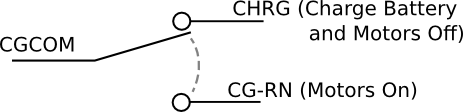
\includegraphics[scale=0.5]{chrg-run-switch}
\caption{The Charge/Run Switch}
\label{fig:chrgrun}
\end{figure}

\subsection{The On/Off switch}
Connect the single-pole-single-throw switch to the \textit{Logic Switch} indicated in the outline. This is the master power switch for your robot.

\subsection{The Powered USB Hub}
Connect the Hub's USB cable to the `Disk2' socket on the side of the slug - see figure \ref{fig:slug-side}. Now attach the SR Power \(\rightarrow\) USB Hub connector. Insert \textbf{both} memory sticks into the USB Hub.

\begin{figure}[h!]
\center
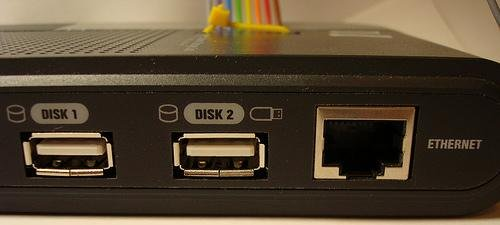
\includegraphics[scale=0.6]{slug-side-view}
\caption{Side view of the Slug's USB Ports}
\label{fig:slug-side}
\end{figure}

\subsection{The Slug}
Identify the Slug's Pin Header on the power board and \textbf{carefully} plug the Slug's multicoloured ribbon cable into it. Be sure to orientate the socket correctly, before applying force. This cable provides both power and data connections between the slug and, indirectly, all the SR modules.

\subsection{The Webcam}
Plug the USB Webcam into the spare USB port on the Slug (Disk1 in figure:\ \ref{fig:slug-side}).

\subsection{RJ11 Cables}
Connect the Motor Board, PWM Board \& JointIO Board to the Power board using three of the supplied, black, RJ11 cables. There will be a spare RJ11 socket on the power board. The order in which they are connected is unimportant. 

\subsection{Motor Board \& Servo Board Power}
Connect your SR power connector from either of the `Motor' sockets on the Power Board, to the power socket on the Motor Board. Connect another SR power connector from the `Servo' socket on the Power board, to the power socket on the PWM Board. You may have to refer to the board-specific documentation. 

These boards have different voltage requirements. Connecting them incorrectly \textbf{will damage your kit}. Be sure to check the polarity matches at both ends of the connector before proceeding to the next step.

\subsection{The Fuse}
Ensure that the fuse is fitted in the fuse socket on the power board before continuing.

\subsection{The battery}
Now attach the battery to the power board using the spade terminals spade connectors. 

\subsection{The Radio Module}
This will be supplied to you on the competition day.


\section{Assembling the Motor Board}
We will now connect the Motor Board to the rest of the kit. Ensure that you have {\bf turned your robot OFF before continuing}

\subsection{RJ11 Cable}
Use one of your RJ11 cables to connect the Power Board (you may use any one of the four RJ11 sockets) to the Motor Board.

\subsection{Motor Power}
Use the wire and SR Connectors to connect the Motor power supply on the Power Board to the socket on the Motor Board. Ensure that the +12V signal at the Power Board is connected to +12V signal at the Motor Board, and also that GND connects to GND. {\bf You will need to refer to the Motor and Power Board Outlines!}

\subsection{Motors}
Now use more wire and SR Connectors to connect your robot's motors to the Motor Board. You will need to refer to the Motor Board Documentation.

\subsection{Testing}
At this point you can write a simple python script to test that the motors are correctly installed. See the Programming Reference for more information


 



\newpage
\section{Assembling the PWM board}
The PWM Board, sometimes referred to as the Servo Board, controls up to 6 Servos and also features an LCD display which can be used during testing. Ensure that you have {\bf turned your robot OFF before continuing}

\subsection{RJ11 Cable}
Use one of your RJ11 cables to connect the Power Board (you may use any one of the four RJ11 sockets) to the PWM Board.

\subsection{Servo Power}
Use the wire and SR Connectors to connect the Servo power supply on the Power Board to the socket on the PWM Board. Ensure that the +5V signal at the Power Board end is connected to +5V signal at the PWM Board end, and also that GND connects to GND. {\bf You will need to refer to the PWM and Power Board Outlines!}

\subsection{Servos}
Refer to the PWM Board Documentation in order to connect your robot's servos to this board.

\subsection{Testing}
At this point you can write a simple python script to test that the servos and LCD are correctly installed. See the Programming Reference for more information.


 



\newpage
\section{Assembling the JointIO board}
The JointIO board provides analogue and digital Input/Output capabilities to your robot. Ensure that you have {\bf turned your robot OFF before continuing}

\subsection{RJ11 Cable}
Use one of your RJ11 cables to connect the Power Board (you may use any one of the four RJ11 sockets) to the JointIO Board.

The JointIO Board draws its power from the RJ11 connection, therefore it does not need an additional power supply.

\subsection{IO Devices}
Refer to the JointIO Board Documentation in order to connect your robot's IO devices to this board.

\subsection{Testing}
At this point you can write a simple python script to echo the value of its inputs at its outputs or to flash its outputs in a simple sequence. This will test that the board has been correctly installed. See the Programming Reference for more information.


 



\section{Conclusion}
Once you have tested each of the boards individually, you should write another python script to test all of the boards together. This will include testing the webcam. It is a very good idea to keep a copy of all of your test routines for use in the future when you make changes which inadvertently stop your robot working.

\newpage
%Glossary of components, terms

\section{Glossary}
\label{sec:glossary}
\begin{longtable}{| l | l| l |}
\hline
\textbf{Component} & \textbf{Description} & \textbf{Quantity} \\ \hline
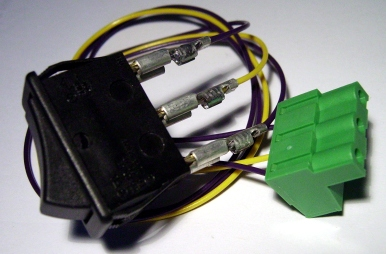
\includegraphics[height=2cm]{chrg-run-sw}  & Charge/Run switch & 1 \\ \hline
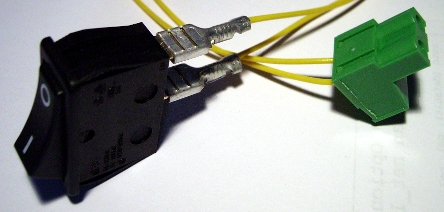
\includegraphics[height=2cm]{on-off-sw}  & On/Off Switch & 1 \\ \hline
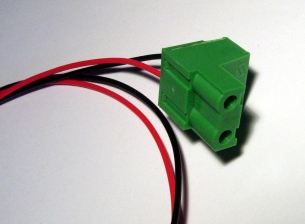
\includegraphics[height=2cm]{battery-con}  & Battery Connector & 1 \\ \hline
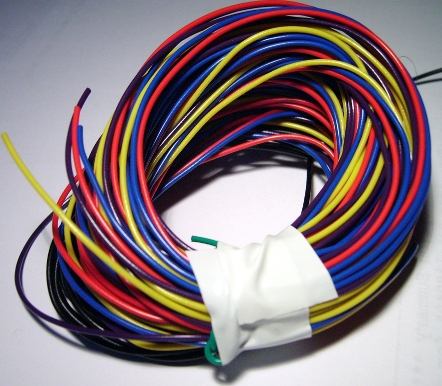
\includegraphics[height=2cm]{wire}  & Multi-core Electrical Wire & 5 \\ \hline
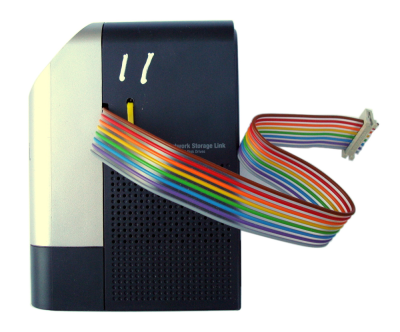
\includegraphics[height=2cm]{slug}  & Slug & 1 \\ \hline
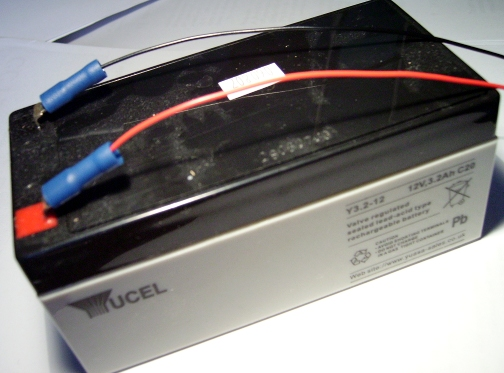
\includegraphics[height=2cm]{battery}  & 12V Sealed Lead Acid battery & 1 \\ \hline
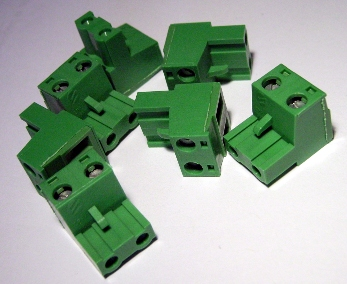
\includegraphics[height=2cm]{camcon}  & SR Connector & 4 \\ \hline
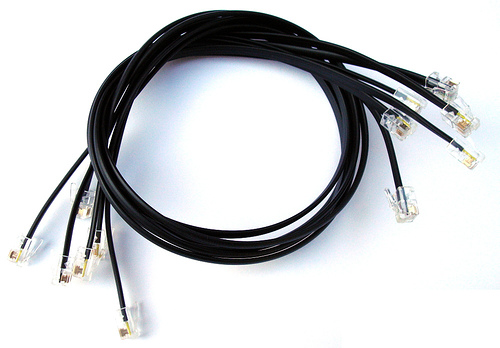
\includegraphics[height=2cm]{4p4c}  & RJ11 Cable & 5 \\ \hline
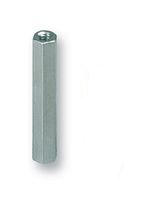
\includegraphics[height=2cm]{spacer}  & PCB Spacers & 17 \\ \hline
-  & USB Memory Stick & 2 \\ \hline
-  & Battery Charger & 1 \\ \hline
- & Web Camera & 1 \\ \hline
- & JointIO Board & 1 \\ \hline
- & Power Board & 1 \\ \hline
- & PWM Board & 1 \\ \hline
- & Motor Board & 1 \\ \hline
 - & USB Hub & 1 \\ \hline
\end{longtable}

\end {document}
